Um einen guten Vergleich und eine Bewertung der verschiedenen umgesetzten Algorithmen anstellen zu können, wurden im folgenden verschiedene interessante Metriken erarbeitet. Es folgt jeweils eine Beschreibung von passenden Testszenarios zur Ermittlung der Metriken und deren zur Auswertung. Anschließend werden die auf diesem Weg entsprechende Graphen für jeden Algorithmus erzeugt und gegenübergestellt.

\subsubsection{Aufbau der Testszenarien}

Die Tests sehen für alle folgenden Testfälle eine Gegenüberstellung der Ausgangssituation vor der Optimierung mit jeweils optimierten Ergebnissen vor. Dafür wird für alle Testfälle eine gleichbleibende Menge von verfügbaren Ressourcen angenommen, welche auf Erfahrungswerten zu benötigten Ressourcen basiert. Dies wäre auch ein nötiges Vorgehen, um am realen Terminal eine sinnvolle Auslastung zu erzielen. Dort wird die Verfügbarkeit aber möglicherweise je nach Personalverfügbarkeit (aus Krankheit, Urlaub etc.) oder Maschinenverfügbarkeit (durch Wartungen, Reparatur etc.) schwanken. Solche besonderen Szenarien werden in späteren Testfällen genauer betrachtet. Zunächst ist es aber der beste Weg, gewöhnliche Szenarien und Abläufe zu vergleichen. Betrachtet werden in allen Tests die zuvor implementierten Verfahren \glqq{}Shortest Job Next\grqq{} (SJN), \glqq{}Most Idle Time\grqq{} (MIT) und \glqq{}First come, first served\grqq{} (FCFS).

Mit folgender Liste von Ressourcen wurde jeweils gearbeitet:
\begin{itemize}
    \item 2x Gabelstapler (Forklift)
    \item 1x Kran (Crane)
    \item 2x Einweiser (Guide)
    \item 2x Fahrer (Driver)
    \item 1x Greifstapler (Reachstacker)
    \item 2x Ketten (Chains)
\end{itemize}

Die Slotgröße wurde in der Regel auf 180 Minuten, also 3 Stunden festgelegt.

Die Listen von verarbeiteten Avisierungen wird für alle Szenarien mit der eigens entwickelten Methode \textit{generateRandomAdvices()} generiert. Sie ermöglicht auch eine Generierung mit ungleicher Verteilung der Abfertigungskategorien der LKW. Für die meisten Testszenarien wird hier eine an die reale Verteilung angelehntes Verhältnis von 2:2:2:1 für LIFT\_CHAINS zu LIFT\_FORKS zu SELF\_DRIVING zu CONTAINER gewählt. \todo{Beibehalten, Quelle woher der Wert kommt}

Die Liste der gebuchten LKW real, wie auch in diesen Tests sehr zufällig. Um das Verhalten und die Streuung der Ergebnisse über viele Durchläufe vergleichen zu können, werden daher alle Werte 100 Mal berechnet und immer die Durchschnittswerte bzw. eine Standardabweichung gezeigt. 

\subsubsection{Testszenario 1: Verhalten mit unterschiedlicher Anzahl von LKW}

Um die Verbesserung durch die Algorithmen zu zeigen, werden die beschriebenen Durchläufe jeweils mit identischen Eingangsparametern, einmal mit dem eigens entwickelten \textit{UnoptimizedScheduler} und einmal mit den jeweiligen Optimierungsalgorithmen durchgeführt. Verglichen werden soll zunächst das Verhalten bei steigender Anzahl von avisierten LKW. Jeder Algorithmus wurde dafür mit einer zufällig generierten Liste von LKWs ausgeführt, wobei die Anzahl der LKW in dieser Liste schrittweise von 1 auf 100 \todo{Warum 100 erklären} erhöht wurde. Da die Ladung der LKW in Realität kaum vorhersehbar und zufällig ist, was auch hier im Test durch eine zufällige Generierung der Eingangsdaten nachgestellt wurde, wird jeder dieser Schritte 100\todo{Warum 100 erklären; 100 auch bei anderen Szenarien einfügen...} Mal mit einer unterschiedlichen Eingangsliste durchgeführt. So ist es möglich, in der nun folgenden Auswertung Durchschnittswerte zu bilden und insbesondere auch Streuungen näher zu betrachten.

Die Werte zu den folgenden Graphen wurden durch die implementierten Testläufe der Testklasse \textit{NumberOfTrucksTest} ermittelt. Alle nachfolgend erklärten Berechnungen und die Erzeugung der Graphen wurden mit dem R Skript \textit{rsNumberOfTrucks.R}\todo{Pfad etc} erzeugt.


\textbf{Verbesserung der Anzahl abgefertigter LKW}

Ziel des gesamten Optimierungsaufwands war es, avisierte LKW effektiv auf einen Slot zu verteilen, sodass möglichst viele LKW abgearbeitet werden können, bzw. dass möglichst wenig Leerlaufzeiten entstehen. Dargestellt wird hier zunächst die prozentuale Verbesserung der Anzahl der erfolgreich eingeplanten LKW (Berechnung siehe Formel \ref{eq:schedJobImpr}) gegenüber der Gesamtanzahl von Buchungen. Ein prozentualer Wert des optimierten Wertes gegenüber dem Unoptimierten gibt in diesem Fall den besten Überblick, wie viel Verbesserung erreicht werden konnte. Die totale Anzahl von LKW kontinuierlich, die Verbesserung wäre hier schwerer zu erkennen.

\begin{equation} \label{eq:schedJobImpr}
schedJobImpr = \left(\dfrac{100}{uScheduledJobs} * oScheduledJobs\right) - 100
\end{equation}

In den Graphen (siehe Abb. \ref{fig:evalAnzahlLkw}) dargestellt wird dabei jeweils der Durchschnittswert über alle 100 Durchläufe, sowie dessen jeweilige einfache Standardabweichung, um ein Maß für die Streuung zu erhalten.

\begin{figure}[H]
\centering
\begin{subfigure}{.495\textwidth}
  \centering
  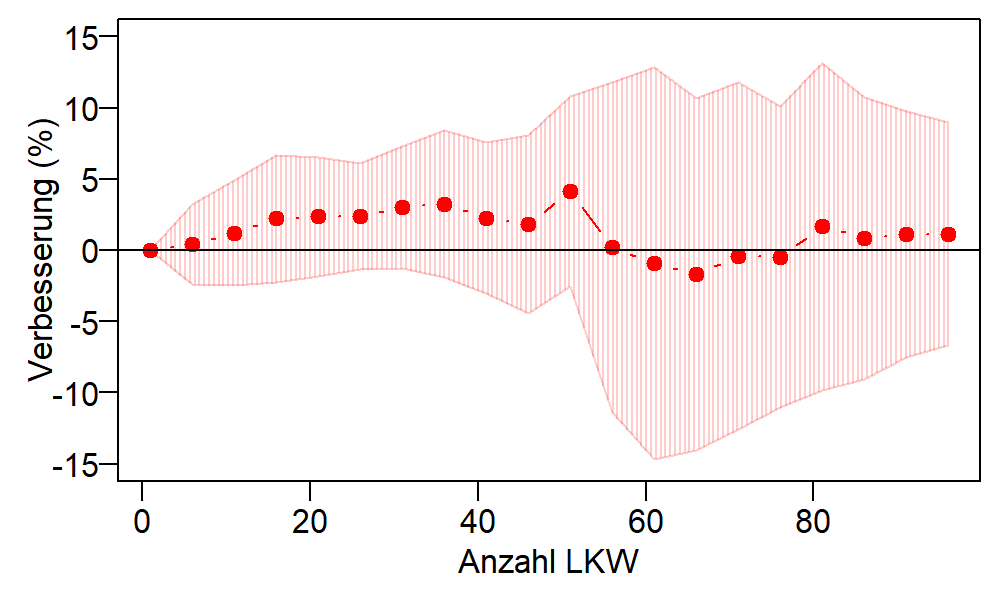
\includegraphics[width=\linewidth]{images/graphs/rsNumberOfTrucksSjn_AnzahlAbgefertigt.png}
  \caption{Shortest Job Next}
  \label{fig:eal1}
\end{subfigure}
\begin{subfigure}{.495\textwidth}
  \centering
  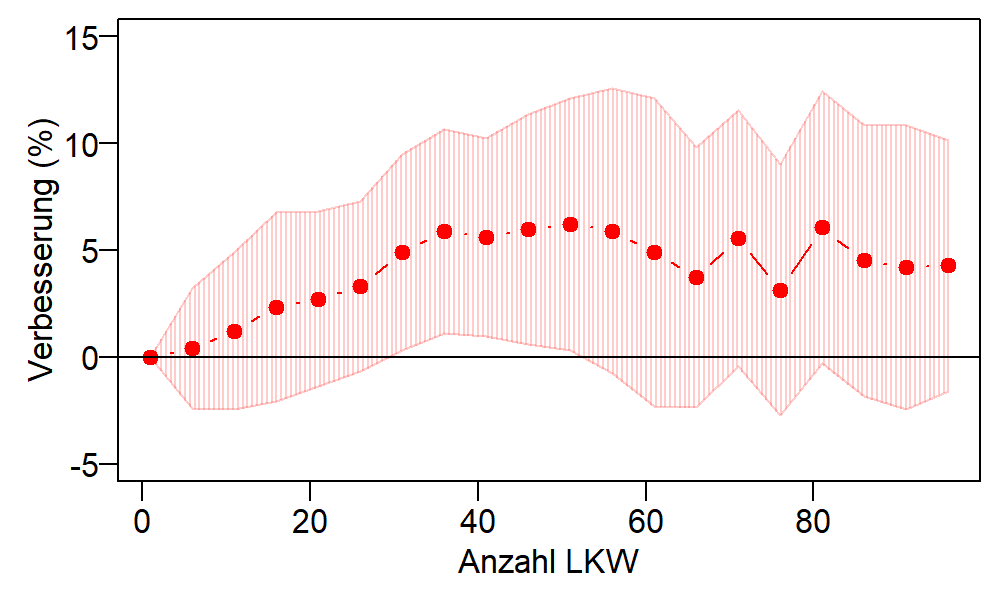
\includegraphics[width=\linewidth]{images/graphs/rsNumberOfTrucksMot_AnzahlAbgefertigt.png}
  \caption{Most Idle Time}
  \label{fig:eal2}
\end{subfigure}

\begin{subfigure}{.5\textwidth}
  \centering
  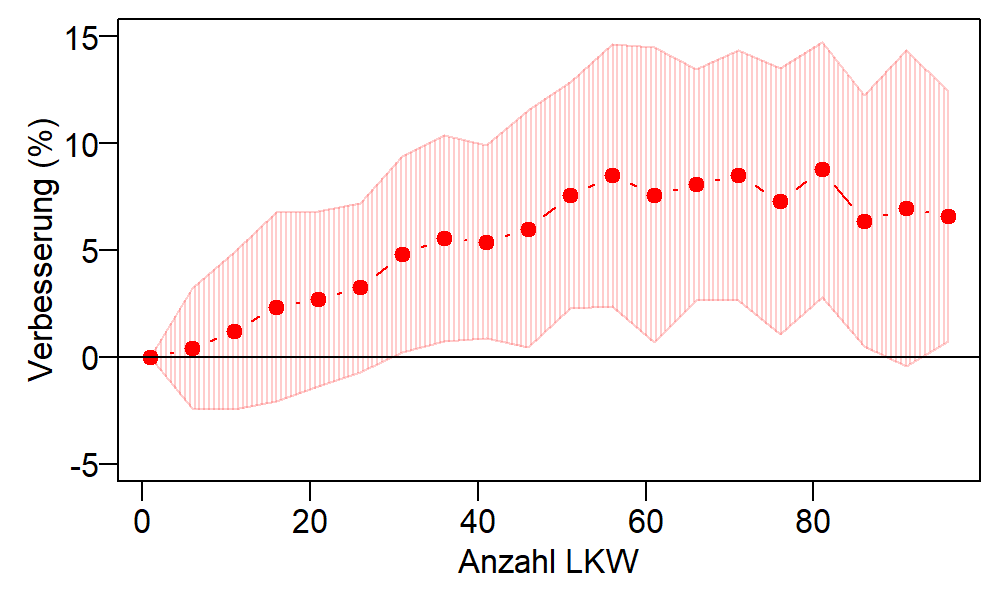
\includegraphics[width=\linewidth]{images/graphs/rsNumberOfTrucksFcfs_AnzahlAbgefertigt.png}
  \caption{First come, first served}
  \label{fig:eal3}
\end{subfigure}

\caption{Verbesserung der Anzahl abgefertigter LKW}
\label{fig:evalAnzahlLkw}
\end{figure}

Was zunächst einmal bei allen Algorithmen auffällig ist, ist dass die Standardabweichung, also die Streuung der Werte sehr hoch ist. Hier ist jeweils die einfache Standardabweichung dargestellt, d.h. geht man von einer Normalverteilung der Werte aus, so liegen in den rot schraffierten Bereichen 68\% der Werte. Eine doppelte Standardabweichung mit 95\% der Werte würde also bei allen Algorithmen im negativen Bereich liegen. Kein Algorithmus garantiert also eine Verbesserung der Werte. Ebenfalls ist bei allen Graphen eine stark sichtbare Veränderung des Anstiegs zwischen 40 und 60 LKW zu erkennen. Dies dürfte etwa die Grenze sein, bei der der 180 Minuten Slot vollgefüllt ist. Bis dort hin bleibt so viel Leerlauf, dass die meisten LKW noch eingeplant werden können, ab dann können die meisten neuen LKW nicht mehr eingeplant werden. Alle Graphen zeigen auch bis etwa 30 LKW eine ähnlich starke Verbesserung von ca. 4-5\%, was darauf zurückzuführen ist, dass in diesem Bereich immer nahezu alle LKW eingeplant werden können und keiner verschoben werden muss.

Auffällig in Graph \ref{fig:eal1} für das Shortest Job Next Verfahren ist allerdings, dass es eine deutlich geringere Verbesserung bei insgesamt größerer Streuung gibt. Bis der Slot bei etwa 50 LKW gefüllt ist, gibt es durchschnittlich eine leichte Verbesserung bis zu etwa 3\%. Die Streuung ist dabei sogar leicht geringer als bei den anderen Algorithmen. Danach fällt die Verbesserung allerdings stark ab und pendelt um 0 herum, teilweise sogar leicht ins negative bei extremer Streuung. Schaut man sich beispielhaft eine grafische Darstellung der Verteilung an (siehe Abb. \ref{}\todo{Beispiel einfügen}), so fällt auf, dass durch die Verplanung der kurzesten Aufgaben am Anfang eine starke Ungleichverteilung entsteht. Zumindest bei den hier gewählten Ladezeiten haben immer die gleichen Abfertigungskategorien auch die kürzesten Ladezeiten, sodass immer die gleichen Ressourcen genutzt werden und im Anschluss andere kaum mehr verplant werden können, weil sie oft parallel mit bereits verplanten Ressourcen vorkommen.

Im Planungsverfahren mit der meisten Leerlaufzeit (siehe Graph \ref{fig:eal2}) lässt sich eine deutlichere Verbesserung erkennen. Bis zur Füllung des Slots bei etwa 40 LKW gibt es eine kontinuierliche Verbesserung bis zu ca. 5\%, bei moderater Streuung. Anschließend pendelt sich die Verbesserung bei 5\% ein, bei allerdings deutlich steigender Streuung. Die anfängliche Steigung dürfte damit zusammen hängen, dass es mit wenigen LKW einfach auch nur möglich ist eine geringe Verbesserung zu erzielen. Je mehr LKW kommen, desto mehr Potenzial kann auch ausgeschöpft werden.

Bei der first come, first served Verteilung (siehe Graph \ref{fig:eal3}) ergibt sich ein sehr ähnliches Bild wie in Graph \ref{fig:eal2}. Bis etwa 40 LKW sind die Steigung und auch die Streuung sehr ähnlich. Allerdings geht die Steigung hier noch bis eta 50 LKW und 7-8\% Verbesserung weiter. Erst dann stagniert diese ebenfalls auch etwa gleichbeibender Höhe und deutlich steigender Streuung.

Bezüglich der Anzahl der möglichen Abfertigungen lässt sich aus dieser Betrachtung schließen, dass die Algorithmen MIT und FCFS für den allgemeinen Fall deutlich besser geeignet sind. Die große Streuung zeigt allerdings auch, dass es sehr große Unsicherheiten bei allen Algorithmen gibt. Dies dürfte vor allem mit der Zufälligkeit der Eingabewerte zusammenhängen. Wenn kaum etwas über die Verteilung der ankommenden LKW bekannt ist, ist es sehr schwierig einen spezialisierten Algorithmus zu finden. Somit kann nur auf allgemein funktionierende Verfahren zurückgegriffen werden, welche dann in der Regel auch Verbesserte Werte liefern. Was allerdings positiv zu bemerken ist, ist dass genau der Wendepunkt zu dem die Slots gefüllt sind, auch der Hochpunkt der Verbesserung ist. Es ergibt aus dieser Betrachtungsweise somit kaum Sinn, Überbuchungen und anschließende Verschiebung einiger LKW in andere Slots vorzunehmen, da es kaum noch Verbesserung bei der Anzahl der verarbeiteten LKW gibt.


\textbf{Verbesserung der Leerlaufzeiten der Ressourcen}

Die Leerlaufzeit der Ressourcen ist, wie erwähnt, ebenfalls von Bedeutung. Je weniger ungenutzte Leerlaufzeit eine Ressource innerhalb des Slots hat, desto mehr wird sie produktiv und wirtschaftlich sinnvoll eingesetzt. Auch hier ist als relatives Maß die prozentuale Verbesserung zwischen den jeweils unoptimierten und optimierten Zeiten aufgetragen. Berechnet wurden diese nach den Formeln \ref{eq:idleImpr} und \ref{eq:idleBestJobsImpr}. Da die Leerlaufzeit bereits in Prozent gespeichert wird, reicht hier die Darstellung der Differenz, um die Verbesserung zu sehen.

\begin{equation} \label{eq:idleImpr}
idleImpr = uIdleTotal - oIdleTotal
\end{equation}
%\begin{equation} \label{eq:idleCompleteImpr}
%idleCompleteImpr = uIdleComplete - oIdleComplete
%\end{equation}
\begin{equation} \label{eq:idleBestJobsImpr}
idleBestJobsImpr = uIdleBetweenJobs - oIdleBetweenJobs
\end{equation}

Die Graphen stellen hier jeweils die Verbesserungen der gesamten Leerlaufzeit, der Leerlaufzeit und die Leerlaufzeit zwischen den einzelnen Jobs dar.

\begin{figure}[H]
\centering
\begin{subfigure}{.495\textwidth}
  \centering
  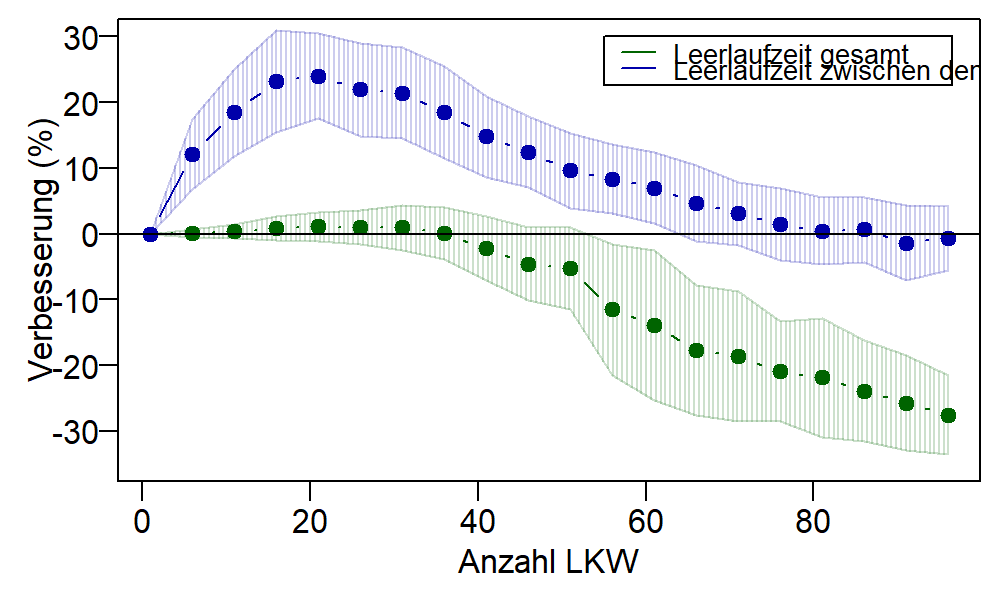
\includegraphics[width=\linewidth]{images/graphs/rsNumberOfTrucksSjn_Leerlaufzeit.png}
  \caption{Shortest Job Next}
  \label{fig:el1}
\end{subfigure}
\begin{subfigure}{.495\textwidth}
  \centering
  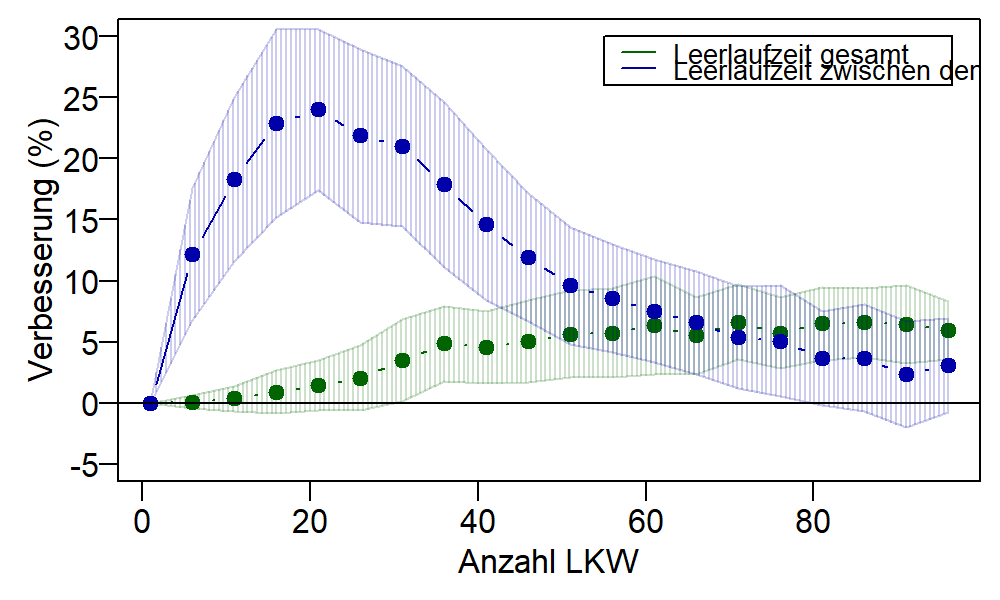
\includegraphics[width=\linewidth]{images/graphs/rsNumberOfTrucksMot_Leerlaufzeit.png}
  \caption{Most Idle Time}
  \label{fig:el2}
\end{subfigure}

\begin{subfigure}{.5\textwidth}
  \centering
  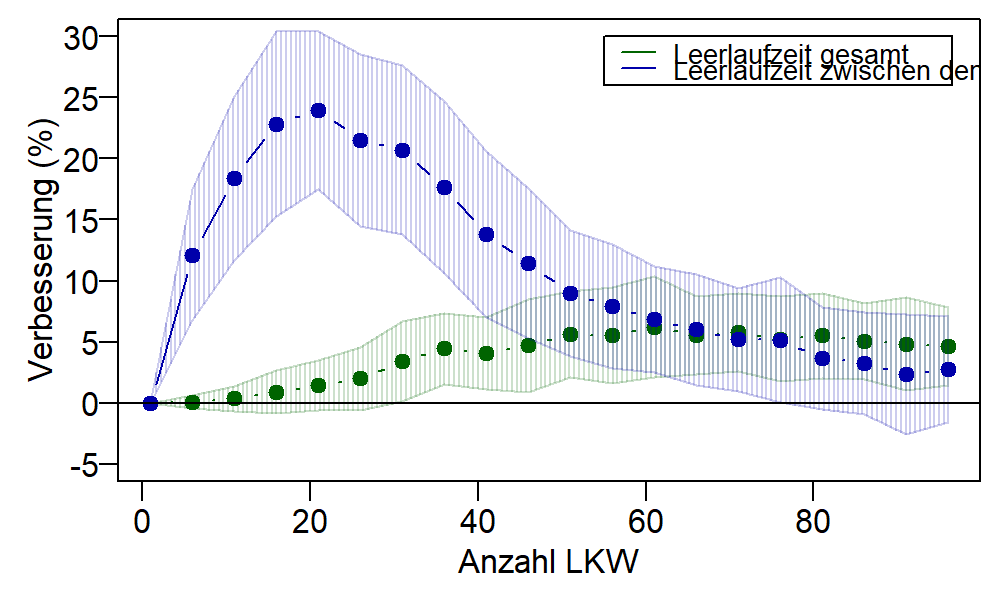
\includegraphics[width=\linewidth]{images/graphs/rsNumberOfTrucksFcfs_Leerlaufzeit.png}
  \caption{First come, first served}
  \label{fig:el3}
\end{subfigure}

\caption{Verbesserung der Leerlaufzeiten der abgefertigten LKW}
\label{fig:evalLeerlaufzeit}
\end{figure}

Mit Blick auf die Leerlaufzeiten lässt sich feststellen, dass die Streuungen hier zwar vorhanden, aber deutlich geringer sind. In den meisten Fällen ergeben sich so keine negativen Verbesserungen bzw. Verschlechterungen der Werte.

In Bezug auf die Leerlaufzeiten schneidet das SJN Verfahren allerdings auch nicht besonders gut ab (siehe Graph \ref{fig:el1}). Die Leerlaufzeiten zwischen den Aufträgen verzeichnen hier zwar eine deutliche Verbesserung von im maximalen Durchschnitt etwa 25\%. Auch die Standardabweichung bis etwa 50-60 LKW so gering, dass es hier so gut wie durchgängig Verbesserungen gegenüber dem unoptimierten Fall gibt. Die Gesamtleerlaufzeit über den Slot verbessert sich allerdings zu Beginn nur ganz minimal und dann zwar auch nur mit sehr geringer Streuung, allerdings verschlechtert sich diese nach dem Füllen des Slots sehr rapide bis zu etwa -25\% bei 100 LKW und einer größer werdenden Streuung. Erklären lässt sich dies in Kombination mit der Anzahl der abgefertigten LKW (siehe Graph \ref{fig:eal1}). Bis der Slot gefüllt ist, lassen sich unoptimiert wie optimiert so gut wie alle LKW unterbringen, somit ergibt sich dort wenig Vorteil bei der Leerlaufzeit. Danach allerdings werden im Durchschnitt gar keine zusätzlichen LKW eingeplant, dafür werden allerdings nach dem Shortest Job Next Prinzip nur die kurzen Aufgaben verplant und die langen fallen heraus und müssen verschoben werden. Insgesamt entsteht aber so eine geringere Auslastung der Ressourcen und somit eine deutliche Verschlechterung, die auch immer weiter ansteigt, je mehr kurze Aufträge es gibt.

Die Verfahren MIT und FCFS unterscheiden sich im direkten Vergleich nur sehr minimal (siehe Graphen \ref{fig:el2} und \ref{fig:el3}). Beide zeigen über den ganzen Zeitraum eine deutlich positive Verbesserung der Leerlaufzeit zwischen den LKW. Diese steigt bis im Durchschnitt etwa 25\% bei 20 LKW an und nimmt dann wieder ab. Um den Bereich zwischen 50 und 60 LKW, wo der Slot wieder komplett ausgefüllt wird, verlangsamt sich diese Abnahme, bleibt aber weiter positiv. Auch unter Berücksichtigung der Standardabweichung ist diese Verbesserung in nahezu allen Fällen positiv. Auch die Gesamtleerlaufzeit lässt eine gute Verbesserung erkennen. Bis etwa 6\% bei 60 LKW steigt diese Zeit bei beiden kontinuierlich an und hält sich dann auf etwa gleichbleibendem Niveau. Die Standardabweichung ist dabei zunächst sehr gering und wird dann bis zum höchsten Niveau immer größer. De größte Teil aller Werte liegt dabei aber immer noch im positiven Bereich, wenn auch deultich geringer als der Durchschnitt.

Schlussfolgern kann man aus dieser Betrachtung, dass das SJN Verfahren zwar für die Verplanung einzelner Ressourcen bezüglich der Leerlaufzeit Vorteile bringt, da die Zeiten zwischen den Ressourcen minimiert werden, über alle Ressourcen betrachtet ergibt sich allerdings kein Vorteil bzw. sogar ein starker Nachteil. Es werden nur kürzere und dabei aber auch nicht mehr Aufträge verplant. Dies bringt nicht nur hier Nachteile, die verschobenen Jobs müssen in späteren Slots zusätzlich eingeplant werden, was dort ebenfalls für große Schwierigkeiten und eine Ungleichverteilung der Auslastungen sorgen wird. Die beiden anderen Verfahren können dagegen allerdings den psoitiven Eindruck der vorherigen Auswertung bestätigen. Bei mehr eingeplanten LKW kann hier gleichzeitig eine geringere Leerlaufzeit verzeichnet werden. Der große Vorteil im Vergleich zu SJN dürfte sein, dass bei beiden Verfahren mehr oder weniger zufällig über alle Abfertigungskategorien hinweg aus den Aufträgen ausgewählt wird. Somit werden die Ressourcen im Schnitt gleichmäßiger ausgelastet und das strukturierte Vorgehen bei der Verteilung kann dann weniger Leerlauf schaffen und so zusätzliche LKW einsetzen.



\textbf{Verbesserung der Wartezeiten je LKW}

Ein Wert, welcher nicht direktes Ziel der Verbesserung war, aber dennoch interessant für eine nähere Betrachtung ist, ist die Entwicklung der Wartezeit der LKW. Lassen sich LKW schneller zu Beginn abarbeiten, kann dies ein Vorteil sein, da LKW Fahrer so nicht so lange ungenutzte Wartezeiten vor oder im Terminal haben und schneller für ihre Speditionen neue Aufträge bearbeiten können.

\begin{equation} \label{eq:avgWaitingImpr}
avgWaitingImpr = \dfrac{uAverageWaitingTime - oAverageWaitingTime}{uAverageWaitingTime} * 100
\end{equation}

\begin{figure}[H]
\centering
\begin{subfigure}{.495\textwidth}
  \centering
  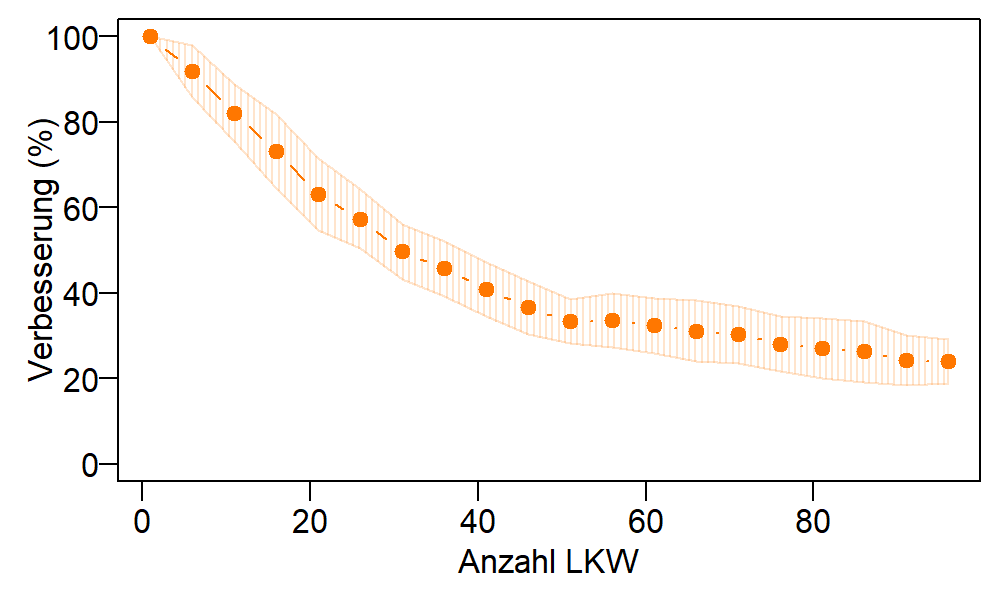
\includegraphics[width=\linewidth]{images/graphs/rsNumberOfTrucksSjn_Wartezeit.png}
  \caption{Shortest Job Next}
  \label{fig:ew1}
\end{subfigure}
\begin{subfigure}{.495\textwidth}
  \centering
  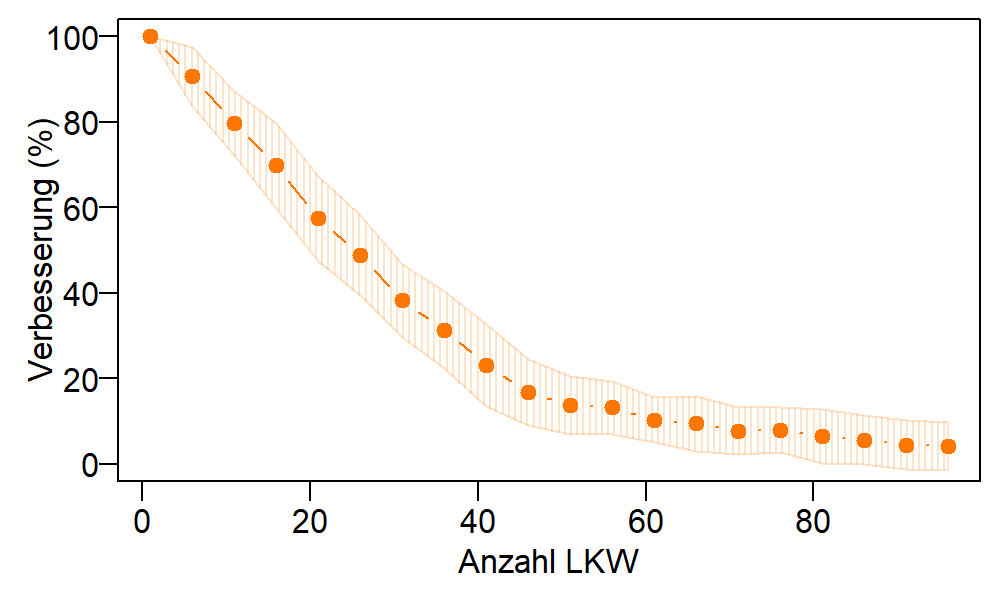
\includegraphics[width=\linewidth]{images/graphs/rsNumberOfTrucksMot_Wartezeit.png}
  \caption{Most Idle Time}
  \label{fig:ew2}
\end{subfigure}

\begin{subfigure}{.5\textwidth}
  \centering
  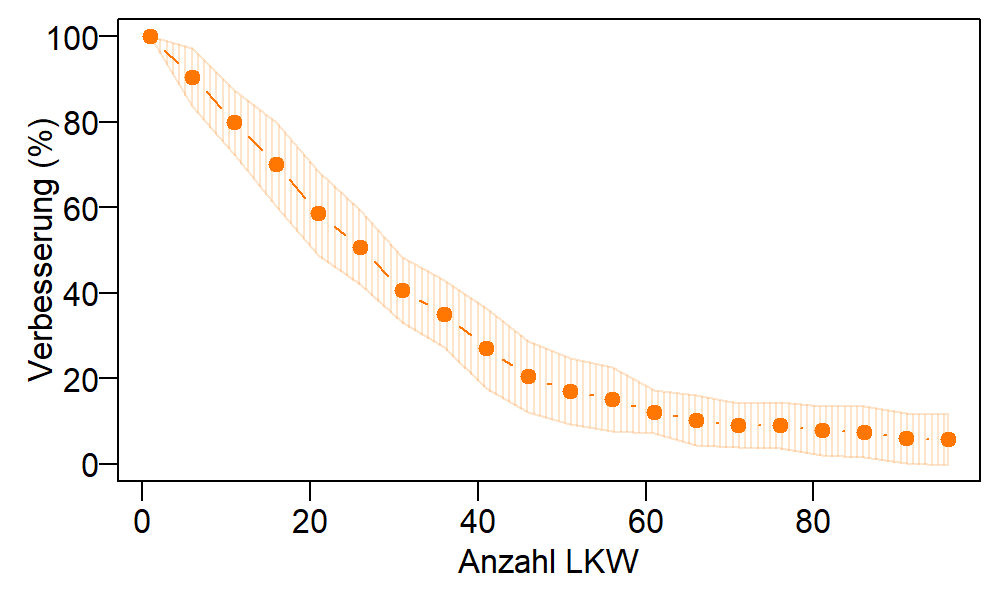
\includegraphics[width=\linewidth]{images/graphs/rsNumberOfTrucksFcfs_Wartezeit.png}
  \caption{First come, first served}
  \label{fig:ew3}
\end{subfigure}

\caption{Verbesserung der Wartezeit der abgefertigten LKW}
\label{fig:evalWartezeit}
\end{figure}

Bei den Wartezeiten ergibt sich ein etwas anderes Bild der betrachteten Verfahren. Alle beginnen bei einer Verbesserung der Wartezeit von 100\%, welche dann überall deutlich sinkt, bis zu dem Punkt wo wieder der gesamte Slot gefüllt ist. Ab diesem Punkt sinkt die Wartezeit überall weiter, allerdings deutlich langsamer. Auch die Streuung ist in diesem Fall sehr gering, sodass es keine Verschlechterungen der Wartezeit gibt.  Die anfänglich sehr große Verbesserung lässt sich darauf zurückführen, dass die LKW im unoptimierten Fall sehr zufällig verteilt über den gesamten Zeitraum des Slots ankommen. So wird jedes Planungsverfahren, welches die Aufgaben so früh wie möglich einplant, zunächst eine deutliche Verbesserung erreichen.

Auffällig ist vor allem, dass die Wartezeit den SJN Verfahrens (siehe Graph \ref{fig:ew1}) langsamer sinkt und sich auch am Ende noch auf einem Niveau von 30-40\% Verbesserung bewegt, während die anderen beiden Fälle (siehe Graphen \ref{fig:ew2} und \ref{fig:ew3}) wieder sehr ähnlich sind und gegen Ende nur noch eine Verbesserung von 10-20\% haben. Dies ist daraum zurückzuführen, dass das SJN Verfahren alle kurzen Aufgaben zuerst einplant, somit können schnell viele LKW abgearbeitet werden, was zu wenig Wartezeit führt. Spätestens, wenn der Slot komplett gefüllt ist und LKW verschoben werden müssen, wird sich der Vorteil dadurch relativieren, dass die verschobenen LKW mit langer Abfertigungszeit in anderen Slots untergebracht werden müssen und damit dort die Wartezeit negativ beeinflussen.

Insgesamt lässt sich aber festhalten, dass in allen Verfahren eine, wenn auch nicht immer allzu hohe Verbesserung erzielt werden kann. Dies war zwar nicht oberstes Ziel der Optimierung, ist allerdings ein schöner und für die LKW Fahrer und Speditionen vorteilhafter Nebeneffekt.



\subsubsection{Testszenario 2: Verhalten bei Überbuchung}

Ein weitere Betrachtungsweise der Algorithmen ist das Verhalten mit zunehmender Anzahl von Buchungen. In diesem Fall wird eine gleichbleibende Liste von Buchungen genutzt, welcher schrittweise LKW hinzugefügt werden. Dies simuliert, dass sich immer weitere LKW Fahrer einen Slot buchen. Interessant ist hier, wie viel Verbesserung sich erzielen lässt, wenn bis zur Auslastungsgrenze des Slots gebucht werden würde und alle weiteren, nicht mehr passenden LKW abgewiesen, bzw. diesen nur noch andere Slots zu Buchung vorgeschlagen werden. Dagegen wäre die Frage, wie viele Überbuchungen man zulassen könnte. Hier würden dann zunächst mehr LKW angenommen, als schaffbar sind. Der Planungsalgorithmus kann dann die für ihn passenden Buchungen nutzen und die restlichen in den nächsten Slot verschieben. Es wurden hier sehr ähnliche Berechnungen, wie im vorherigen Testszenario angewendet, auch hier wird ein Vergleich von simulierten, unoptimierten Zustand zu den Ergebnissen der verschiedenen Algorithmen vorgenommen.

Die Werte der folgenden Auswertung wurden durch die Testklasse \textit{OverfillTest} erzeugt. Alle anschließenden Berechnungen und Graphen sind mit dem R Skript \textit{rsOverfill.R}\todo{Pfad etc} berechnet worden.

Die Graphen (Abb. \ref{fig:evalOverfill}) zeigen in diesem Fall jeweils die absolute Anzahl an tatsächlich geplanten LKW im unoptimierten Zustand (blau) und im optimierten Fall (rot). So ist in hier deutlicher erkennbar, wann nicht mehr alle LKW eingeplant werden können, wann also Überbuchungen stattfinden müssten. Die diagonale Gerade mit einer Steigung von 1 zeigt dabei den Fall eines unbegrenzten Slots, sodass jeder LKW, welcher gebucht wurde auch verarbeitet werden kann. Im Verhältnis dazu wird auf der zweiten y-Achse die Verbesserung der Leerlaufzeit aufgetragen. Die Zeit zwischen den LKW in orange und die Gesamtleerlaufzeit in grün. Diese wurden wieder nach dem gleichen Weg wie im ersten Testszenario berechnet (siehe Formeln \ref{eq:idleImpr} und \ref{eq:idleBestJobsImpr}). So lässt sich ein direkter Vergleich anstellen, bei wie viel Buchungen die effektivste Ausnutzung des Slots erreicht wird.


\begin{figure}[H]
\centering
\begin{subfigure}{.495\textwidth}
  \centering
  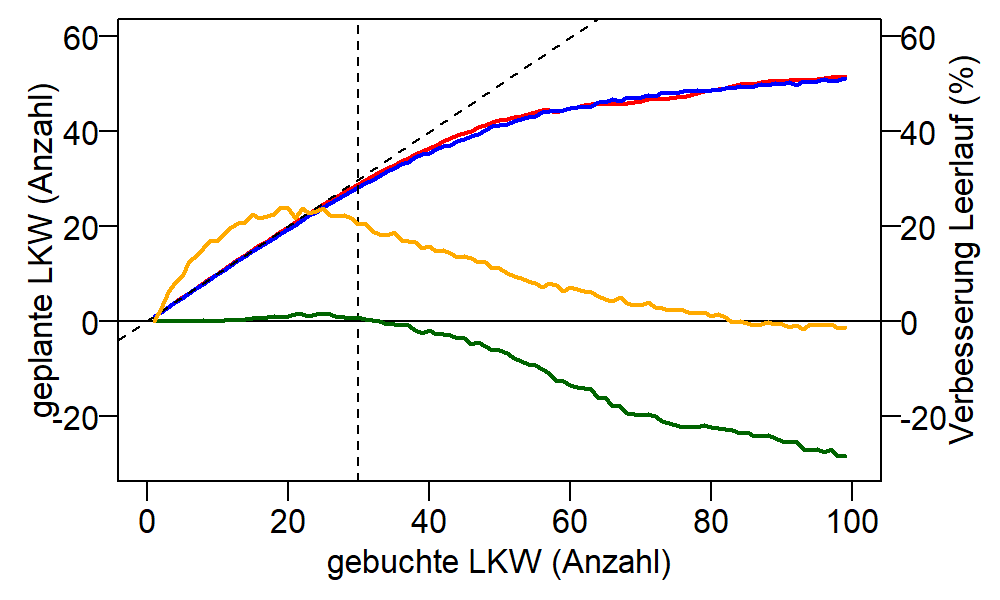
\includegraphics[width=\linewidth]{images/graphs/rsOverfillSjn.png}
  \caption{Shortest Job Next}
  \label{fig:eof1}
\end{subfigure}
\begin{subfigure}{.495\textwidth}
  \centering
  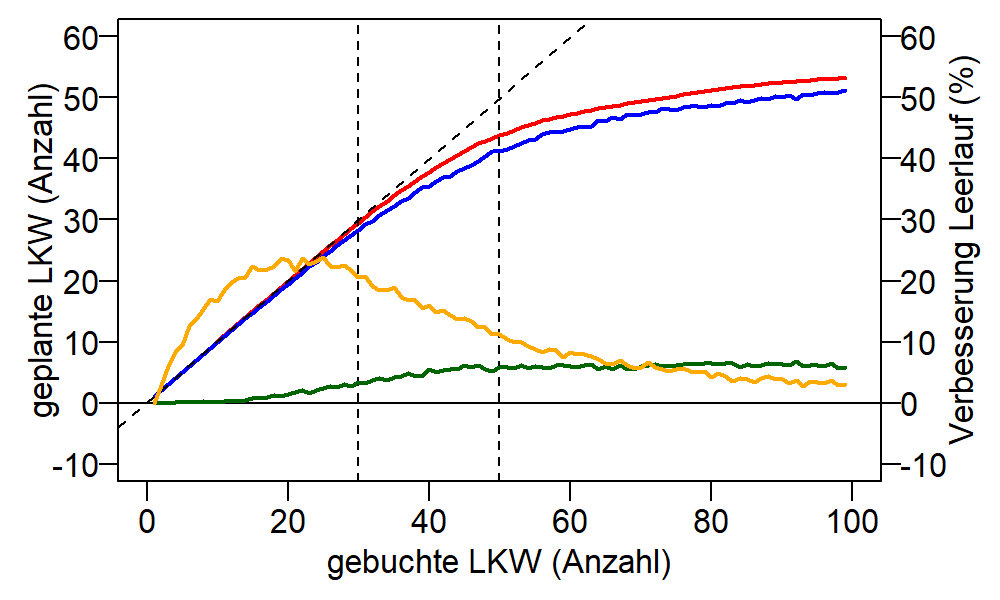
\includegraphics[width=\linewidth]{images/graphs/rsOverfillMit.png}
  \caption{Most Idle Time}
  \label{fig:eof2}
\end{subfigure}

\begin{subfigure}{.5\textwidth}
  \centering
  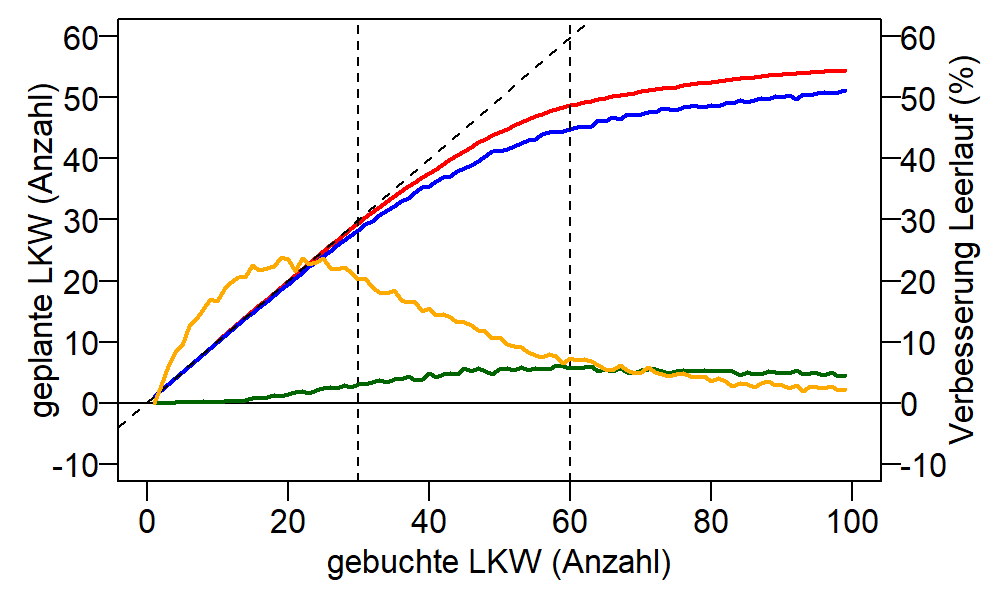
\includegraphics[width=\linewidth]{images/graphs/rsOverfillFcfs.png}
  \caption{First come, first served}
  \label{fig:eof3}
\end{subfigure}
\caption{Verhalten bei Überbuchung}
\label{fig:evalOverfill}
\end{figure}
\todo{Zuklein?, Legende?!}

Erkennbar ist zunächst einmal bei allen Darstellungen, dass überall die Anzahl der eingeplanten LKW bei etwa 30 anfängt, von der diagonalen für den unbegrenzten Slot abweicht. Dies ist also bei allen der Punkt, wo im Durchschnitt langsam nicht mehr alle LKW in den Slot passen. Verdeutlicht wird dieser Punkt in allen Graphen durch die erste senkrechte Linie.

Im SJN Verfahren (siehe Graph \ref{fig:eof1}) halten sich die beiden Anzahlen der eingeplanten LKW sehr nah beieinander, es gibt also im Durchschnitt kaum Verbesserungen oder Verschlechterungen. Die Gesamtleerlaufzeit verschlechtert sich ganz zu Beginn leicht und Verbessert sich dann bis zur markanten Grenze von 30 LKW leicht. Anschließend fällt sie rapide ab, wie es auch schon im vorherigen Szenario sichtbar war. Fängt man hier also an zu überbuchen, werden im Durchschnitt nicht mehr LKW abgefertigt, dafür steigt aber die Leerlaufzeit massiv. 

Auch in diesem Beispiel wiesen die Graphen der Verfahren MIT und FCFS (Abb. \ref{fig:eof2} und \ref{fig:eof3}) deutliche Ähnlichkeiten auf. Hier lässt sich allerdings ab 30 LKW ein größerer Anstieg der geplanten LKW im optimierten Fall erkennen, als es unoptimiert der Fall ist. Auffällig ist aber, dass die Steigung bei MIT schon bei etwa 50 LKW anfängt, deutlicher zu sinken, während es im FCFS Verfahren erst bei etwa 60 LKW der Fall ist (vgl. die zweite senkrechte Linie in den jeweiligen Graphen). Dies ist auch jeweils der Punkt, wo der Abstand zwischen der roten und der blauen Linie nicht mehr größer wird und somit auch kaum noch eine Verbesserung in der Anzahl der abgefertigten LKW stattfindet. Gleichzeitig ist dies auch der Punkt, an dem die Steigung bei der Verbesserung der Gesamtleerlaufzeit stagniert. Auch die Verbesserung Leerlaufzeit zwischen den den Aufträgen nähert sich ab da der Null an. 

Für die beiden Planungsverfahren MIT und FCFS kann man also festhalten, dass gewisse Überbuchung durchaus von Vorteil ist. Für den dreistündigen Slot, welcher ohne Überbuchung schon bei ca. 30 LKW gefüllt wäre, kann man durchaus eine Überbuchung im Bereich von 50-100\%, also insgesamt 45 bis 60 LKW zulassen. Dies führt zu einer deutlich optimierten Auslastung des Slots. Während im SJN Verfahren eine Verschiebung bedeuten würde, dass auch in nachfolgenden Slots eine Ungleichverteilung stattfinden würde, würde sich eine Verschiebung hier vermutlich nicht wirklich negativ auswirken. Da die Verteilung der Abfertigungskategorien, wie bereits festgestellt, ohnehin sher gleichmäßig ist, würde auch eine gleichmäßig durchmischte Liste verschoben. Darüber hinaus lässt sich eben bei einer Überbuchung eine deutlich verbesserte Auslastung und verringerte Leerlaufzeit erzielen, welche bei strikter Begrenzung der Buchungen sehr sehr viel geringer ausfallen wird.


\subsubsection{Testszenario 3: Verhalten bei unterschiedlicher Slotgröße}
\todo{Leerlaufzeit vergleichen?}

In diesem Test soll nun im Gegensatz zu den Vorherigen die Slotgröße variiert werden. Die bisherige Größe wurde mit 180 Minuten gewählt, da sich so eine höhere Anzahl und \glqq{}Auflösung\grqq{} bei den gebuchten LKW ergibt. Bei sehr kleinen Slots lassen sich noch weniger signifikante Veränderungen bis zur Slotsgrenze darstellen, wie auch der folgende Test zeigt. \todo{Ist das wirklich so, prüfen, wenn geschrieben...} Zu analysieren ist hier, wie sich die Anzahl der geplanten LKW und die Leerlaufzeiten verbessern, wenn kleinere oder größere Slots verwendet werden. Dies ist auch für den realen Einsatz sehr interessant, um das beste Verhältnis zwischen möglichst guter Optimierung und den Bedürfnissen der LKW Fahrer und Speditionen zu finden.

Die Werte für dieses Szenario wurden mit den Implementierungen aus der Testklasse \textit{SlotsizeTest} berechnet. Mit dem R Skript \textit{rsSlotsize.R} \todo{Pfad etc.} wurden alle Graphen und Berechnungen erzeugt.

Dargestellt werden in den Auswertungen jeweils wieder die prozentuale Verbesserung bei der Anzahl der eingeplanten LKW. Zur Berechnung wurde wieder die Formel \ref{eq:schedJobImpr} genutzt. Dabei entspricht jede Linie einer anderen Slotgröße.

\begin{figure}[H]
\centering
\begin{subfigure}{.495\textwidth}
  \centering
  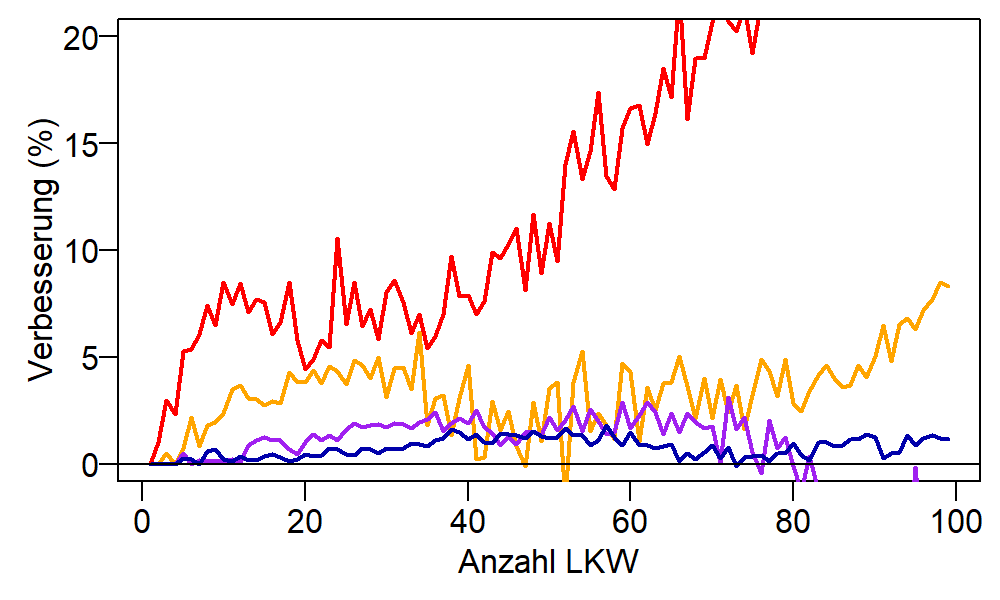
\includegraphics[width=\linewidth]{images/graphs/rsSlotsizeSjn.png}
  \caption{Shortest Job Next}
  \label{fig:eof1}
\end{subfigure}
\begin{subfigure}{.495\textwidth}
  \centering
  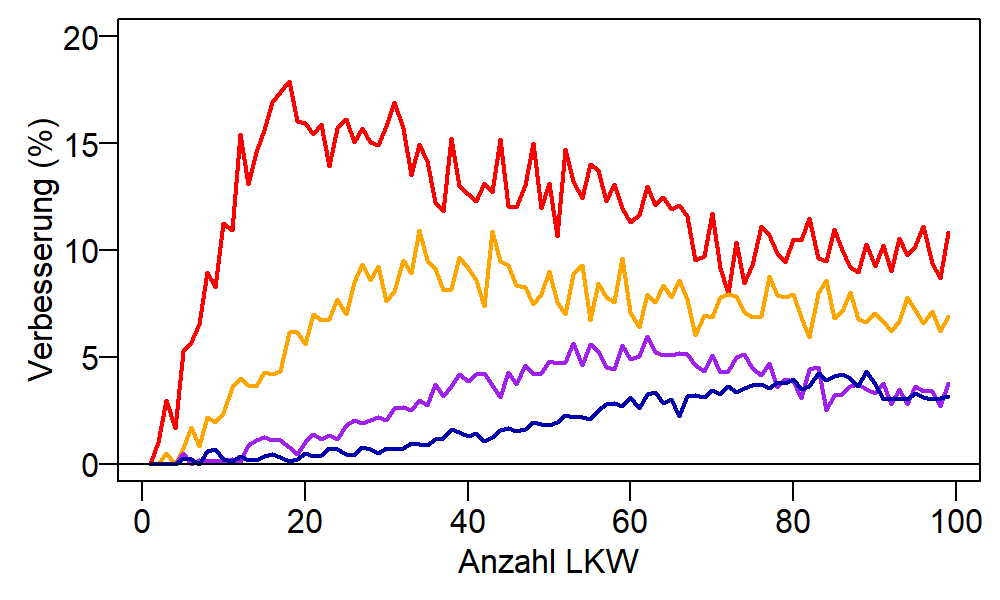
\includegraphics[width=\linewidth]{images/graphs/rsSlotsizeMit.png}
  \caption{Most Idle Time}
  \label{fig:eof2}
\end{subfigure}

\begin{subfigure}{.5\textwidth}
  \centering
  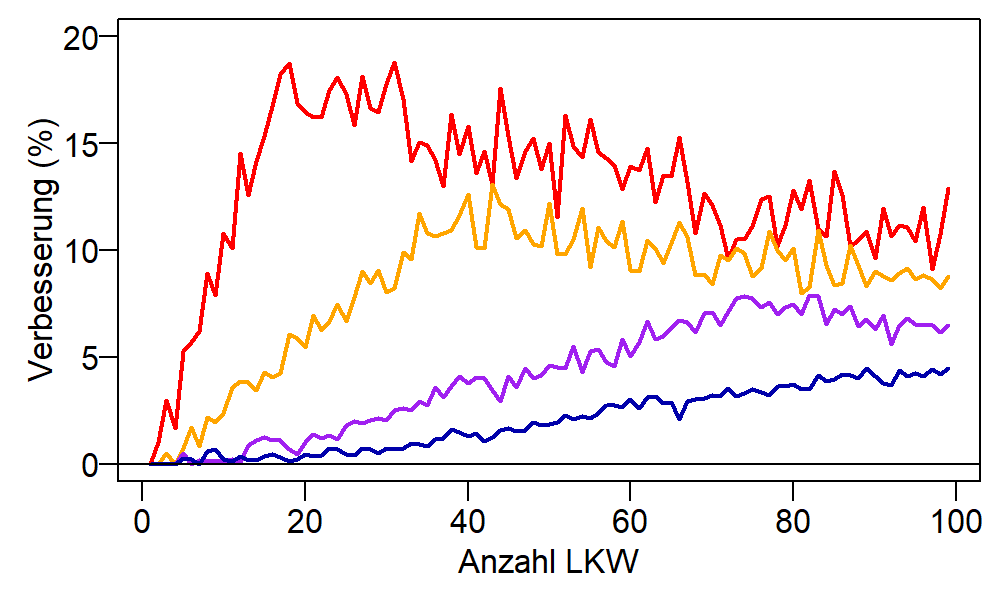
\includegraphics[width=\linewidth]{images/graphs/rsSlotsizeFcfs.png}
  \caption{First come, first served}
  \label{fig:eof3}
\end{subfigure}
\caption{Verbesserung der geplanten LKW bei veränderter Slotgröße}
\label{fig:evalSlotsize}
\end{figure}
\todo{Zuklein?, Legende?!, evtl. auch nicht Verbesserung sondern oScheduled zeigen, wegen streuung?!}

\begin{figure}[H]
\centering
\begin{subfigure}{.495\textwidth}
  \centering
  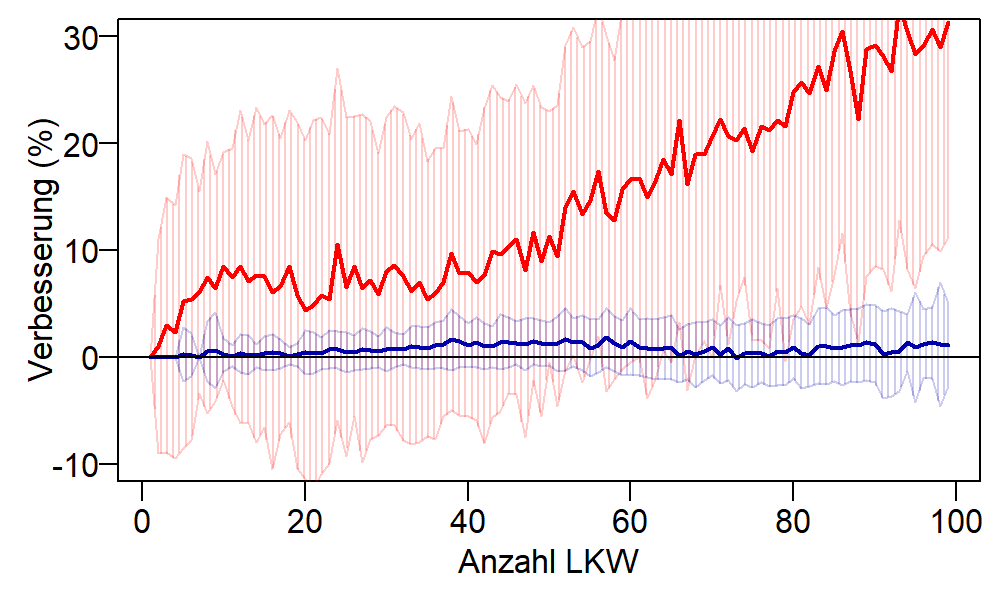
\includegraphics[width=\linewidth]{images/graphs/rsSlotsizeSjn_Streuung.png}
  \caption{Shortest Job Next}
  \label{fig:eofs1}
\end{subfigure}
\begin{subfigure}{.495\textwidth}
  \centering
  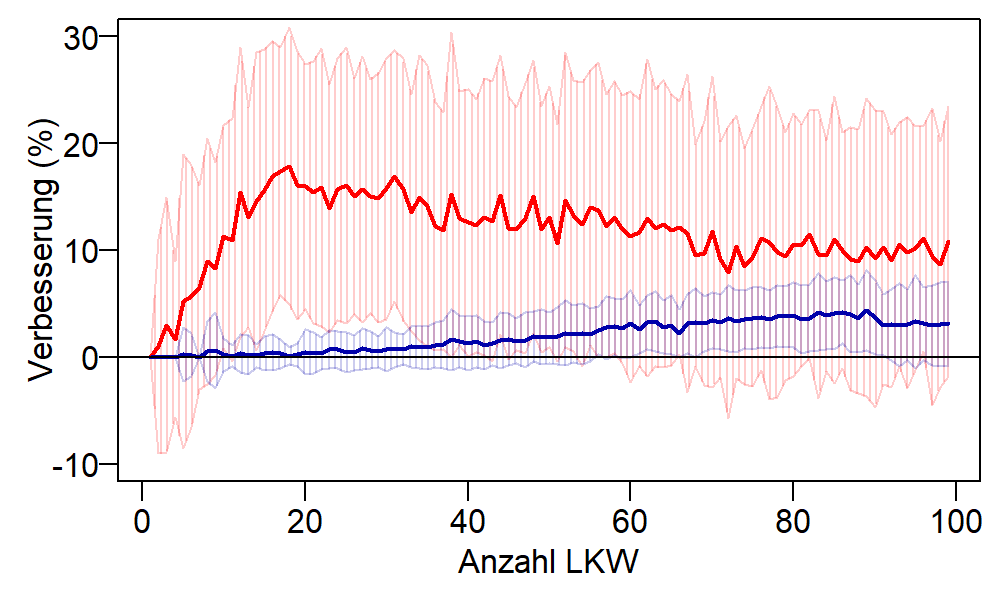
\includegraphics[width=\linewidth]{images/graphs/rsSlotsizeMit_Streuung.png}
  \caption{Most Idle Time}
  \label{fig:eofs2}
\end{subfigure}

\begin{subfigure}{.5\textwidth}
  \centering
  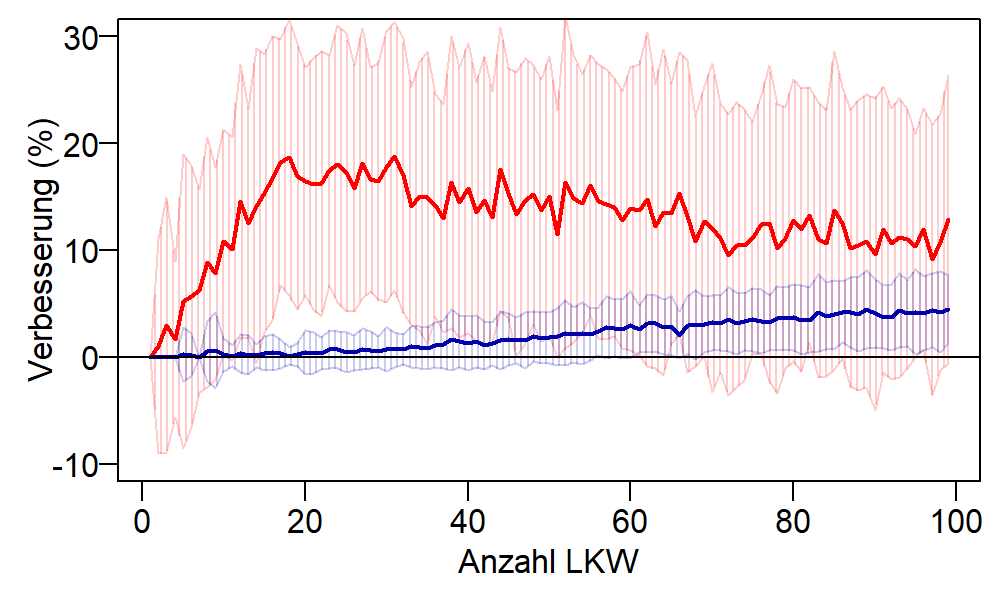
\includegraphics[width=\linewidth]{images/graphs/rsSlotsizeFcfs_Streuung.png}
  \caption{First come, first served}
  \label{fig:eofs3}
\end{subfigure}
\caption{Streuung der Verbesserung der geplanten LKW bei veränderter Slotgröße}
\label{fig:evalSlotsizeStreuung}
\end{figure}
\todo{Zuklein?, Legende?!}

Eine Betrachtung der Testergebnisse (siehe Abb. \ref{fig:evalSlotsize}) zeigt hier tatsächlich unerwartet große Unterschiede auf. In der Gesamtsicht lässt sich schon auf den ersten Blick fetsthalten, dass eine Veränderung der Slotgröße erheblichen Einfluss auf die Verbesserungsrate hat. 

Der Eindruck, dass das SJN Verfahren eher keine allzu guten Ergebnisse liefert, setzt sich hier fort. Die Streuung der Werte ist sehr hoch, insbesondere bei kleinen Slots (siehe Graphen \ref{fig:evalSlotsizeStreuung}). Bei 60 Minuten Slotgröße ist noch eine relativ hohe Verbesserung zwischen 5 und 10\% zu erkennen, welche ab ca. 40 LKW auch noch einmal extrem weiter ansteigt. Je größer die Slots allerdings werden, desto geringer oder sogar negativer wird die Verbesserung. Man könnte nun sagen, dass die Verbesserung beim 60 Minuten Slot wirklich gut ist. Allerdings wurde in den vorherigen Szenarien bereits festgestellt, dass sich eine Überbuchung insgesamt sehr negativ auswirkt. Der extreme Anstieg der Verbesserung kann also gar nicht genutzt werden, da nur die ersten 10-15 LKW wirklich sinnvoll eingeplant werden können. Alle weitere Verbesserung ist nicht nutzbar, da so extrem viele LKW auf andere Slots verschoben werden müssten und sind dann dort sehr negativ auswirken. Auch die hohe Streuung der Werte sprich nicht gerade für ein gutes Verfahren, da kaum konstant positive Ergebnisse erzeugt werden.

Anders sieht es dagegen wieder bei den beiden anderen Verfahren aus. Auch hier lassen sich wieder große Ähnlichkeiten zwischen den Auswertungen der beiden Verfahren feststellen. In allen Kurven ist ein starker Anstieg bis zu einem Maximum zu erkennen und ein anschließender, leichterer Abfall der Verbesserung. Diese Spitze verschiebt sich mit steigender Größe der Slots nach hinten, was auf die größere Kapazität für LKW zurückzuführen ist. Sehr auffällig ist, dass es bei kleineren Slots deutlich höheres Verbesserungspotenzial gibt. Im 60 Minuten Slot erreicht das MIT Verfahren im Durchschnitt bis zu ca. 17\% Verbesserung und das FCFS Verfahren sogar noch mit durchschnittlich etwa 18\% in der Spitze sogar noch etwas mehr. Im 120 Minuten Slot sind es nur noch maximal etwa 11 respektive 13\% in der Spitze. In den weiteren Schritten ist die Abnahme nicht mehr ganz so hoch, aber immer noch sichtbar. Allerdings ist auch in diesen beiden Verfahren die Streuung, gerade bei kleinen Slots sehr hoch (siehe Graphen \ref{fig:eofs2} und \ref{fig:eofs3}).

Schlussfolgernd aus diesem Test lässt sich sagen, dass bei Nutzung der Verfahren MIT oder FCFS durchaus eine kleinere Slotgröße empfehlenswert ist. Was tatsächlich ein sehr spannendes Ergebnis ist. Durch die extreme Streuung gibt es hier durchaus Potenzial für große Verbesserungen, allerdings sind auch sehr geringe Unterschiede zum unoptimierten Fall möglich. In vorherigen Betrachtungen hätte man durchaus zu der Vermutung kommen können, dass größere Slots durch die größere Anzahl von möglichen LKW und somit größeren Planungsspielraum, ein größeres Optimierungspotenzial und somit bessere Ergebnisse liefern. Es ist allerdings auch zu bemerken, dass die Planungsalgorithmen mit steigender Größe der Slots nicht unbedingt schlechter bzw. weniger gut werden. Ein großer Faktor dürfte hier auch sein, dass das bisherige, unoptimierte Verfahren für kleine Slots sehr ungeeignet ist\todo{Das nochmal irgendwo zeigen/belegen?}. Gerade bei kleinen Slots ist eine zufällige Ankunftszeit innerhalb des Zeitraums sehr problematisch, da vor allem am Anfang sehr viele Leerlaufzeiten entstehen, welche sich erst sehr viel später ausgleichen können, wenn mehr LKW warten. Bei kleinen Slots würden dann sehr viel schneller LKW aus dem Zeitfenster herausfallen. Dies führt bei größer werdenden Slots natürlich zu sehr viel mehr abgefertigten LKW und einer besseren Auslastung, die Wartezeiten werden dann aber natürlich hoch sein. Diese hohe Variabilität und der kleine Spielraum bei der Planung führt eben zu dieser hohen Streuung der Werte.


\subsubsection{Testszenario 4: Verhalten bei ungleicher Verteilung benötigter Ressourcen}

Der letzte Eingangsparameter, welcher das Optimierungsergebnis stark beeinflussen dürfte, ist die Art und Anzahl der verfügbaren Ressourcen, bzw. die Verteilung der Art der Ladungen und somit der Bedarf an Ressourcen. Bisher wurde hier immer mit einer ausgeglichenen Verteilung der Ladungsarten gearbeitet und auch die Art und Anzahl der verfügbaren Ressourcen war relativ gut an diesen Fall angepasst. Die Frage die sich nun stellt ist, wie sich die Algorithmen und Optimierungsergebnisse verhalten, wenn hier eine starke Ungleichverteilung herrscht, d.h. wenn sehr viele Ladungen des gleichen Typs ankommen, dann aber keine dazu passende Anzahl von Ressourcen und Ladehilfsmitteln bereitsteht. 

Zu diesem Zweck wurden in diesem Fall die verfügbaren Ressourcen so gelassen, wie sie zuvor auch verwendet wurden, allerdings wurde nun die Anzahl der Buchungen der Kategorie LIFT\_CHAINS schrittweise im Verhältnis zu den übrigen Kategorien erhöht. Die Wertetabellen wurden hier mit der Testklasse \textit{CategoryDistributionTest} erzeugt und mittels des R-Skripts \textit{rsCategoryDistribution.R} \todo{Pfad, etc} ausgewertet. Jeweils dargestellt werden die Ergebnisse für eine Gleichverteilung von 1:1:1:1 und die Verteilungen 3:1:1:1 bzw. 5:1:1:1. Auch hier wurde wieder mit der absoluten Zahl der verplanten LKW gearbeitet, da so die Streuung im unoptimierten Zustand keinen zu großen Einfluss auf die optimierten Werte hat. Jeweils zu erkennen sind die optimerten Werte in der kräftigeren Farbe und zum Vergleich die unoptimerten Durchschnitte in einer etwas helleren Farbe.


\begin{figure}[H]
\centering
\begin{subfigure}{.495\textwidth}
  \centering
  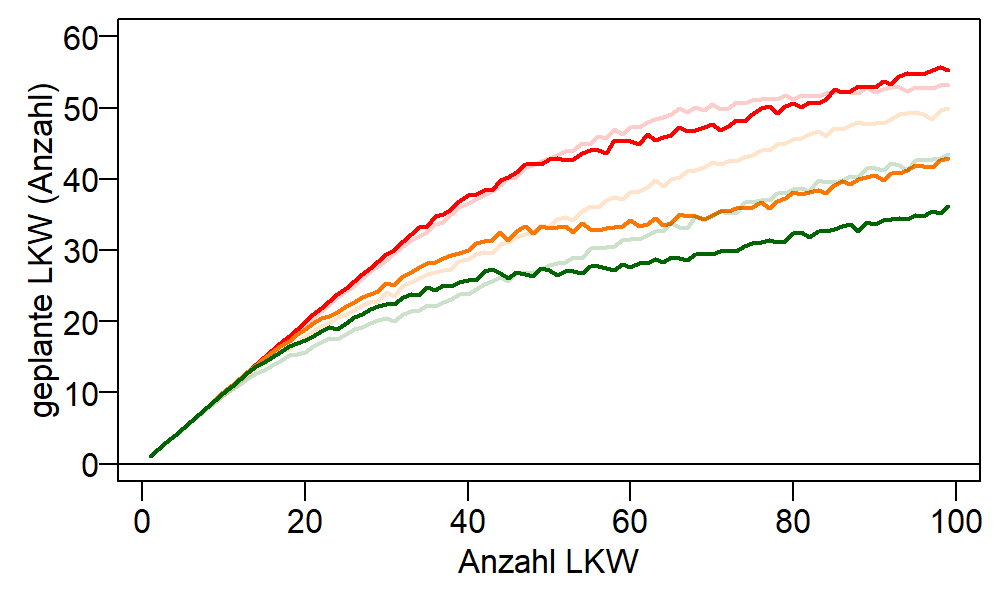
\includegraphics[width=\linewidth]{images/graphs/rsCategoryDistributionSjn.png}
  \caption{Shortest Job Next}
  \label{fig:ecd1}
\end{subfigure}
\begin{subfigure}{.495\textwidth}
  \centering
  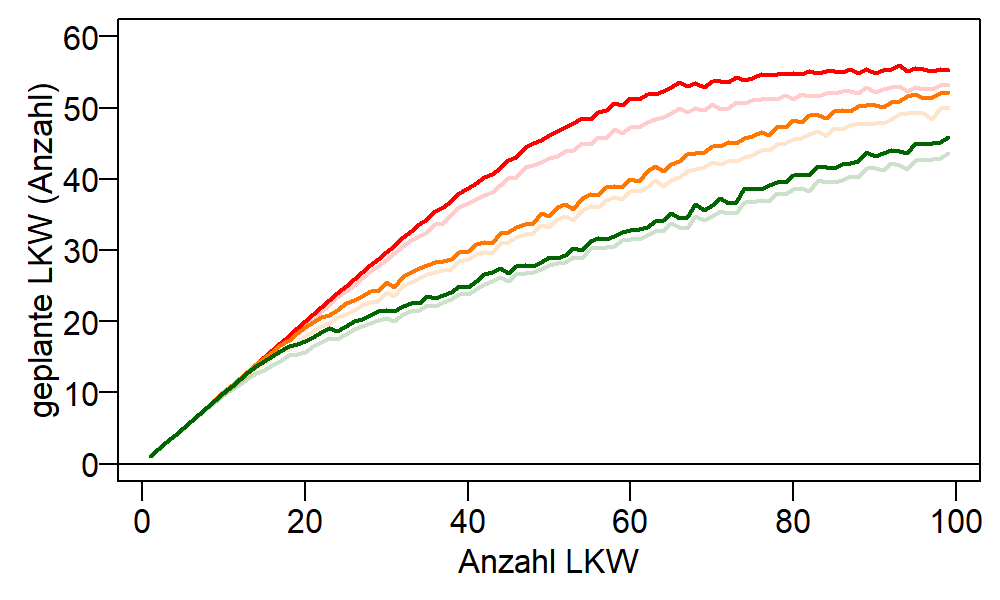
\includegraphics[width=\linewidth]{images/graphs/rsCategoryDistributionMit.png}
  \caption{Most Idle Time}
  \label{fig:ecd2}
\end{subfigure}

\begin{subfigure}{.5\textwidth}
  \centering
  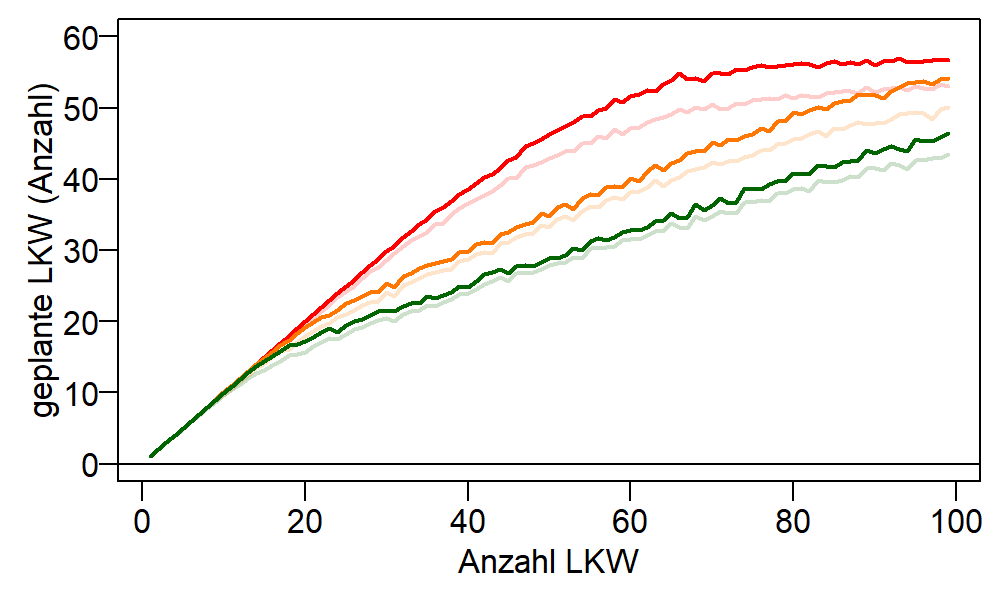
\includegraphics[width=\linewidth]{images/graphs/rsCategoryDistributionFcfs.png}
  \caption{First come, first served}
  \label{fig:ecd3}
\end{subfigure}
\caption{Geplante LKW bei steigender Ungleichverteilung der Abfertigungskategorien}
\label{fig:evalCategoryDist}
\end{figure}
\todo{Legende}

Auch dieses letzte Testszenario verfestigt das Bild und die Bewertung, welche schon zuvor über die einzelnen Verfahren gewonnen wurde. 

Das SJN Verfahren (siehe Graph \ref{fig:ecd1}) zeigt wie auch schon zuvor festgestellt wenig Verbesserung und sogar eine teilweise Verschlechterung der Anzahl der abgefertigten LKW. Extremer wird dieses Verhalten sogar, bei der hier gezeigten Ungleichverteilung. Gegenüber der ausgeglichenen Verteilung ergibt sich hier zunächst ein starker negativer Sprung, aber auch gegenüber der jeweils unoptimierten Kurve sind hier starke Verschlechterungen erkennbar. Je ungleicher die Verteilung wird, das Ergebnis aber nicht mehr ganz so viel schlechter. Es ist allerdings auch zu erkennen, dass die Verbesserung gegenüber dem unoptimierten Fall im unteren Bereich zwischen etwa 20 und 40 LKW leicht steigt, wenn die Verteilung unausgeglichener ist. Insgesamt war dieses Verfahren aber ohnehin schon kein Favorit für einen realen Einsatz, spätestens aber wenn keine gute Prognose der Verteilung der ankommenden LKW möglich ist und somit keine dazu passenden Ressourcen zur Verfügung gestellt werden können, verschlechtert sich die Performance stark.

Die Verfahren MIT und FCFS, verhalten sich hier wie auch schon in den vorherigen Auswertungen sehr ähnlich, wie Graphen \ref{fig:ecd1} und \ref{fig:ecd2} zeigen. Auch hier hat FCFS mit höherer Zahl von LKW wieder leicht höhere Werte als MIT. Erkennbar ist, dass die Anzahl der erfolgreich eingeplanten LKW deutlich sinkt, wenn es eine stärkere Ungleichverteilung gibt. Gleichzeitig nimmt auch die Verbesserung gegenüber dem unoptimerten Fall ab. Im für einen 180 Minuten Slot interessanten Fall bis ca. 60 LKW erreicht der Unterschied der Kurven sein Maximum. Dass sich der Nachteil dieser Verteilung mit noch weiter steigender Zahl wieder verringert, ist also in der Realität weniger relevant. Es lässt sich daraus schließen, wie auch schon zu erwarten war, dass es schon im vorhinein das Ziel sein sollte, eine möglichst gute Prognose der ankommenden LKW zu haben, zumindest was die Verteilung der Ladungstypen angeht. Wenn einfach keine passenden Aufträge für die zur Verfügung stehenden Maschinen hereinkommen, kann auch der beste Algorithmus keine gute Auslastung aller Ressourcen erzeugen. Dennoch erkennt man, dass beide Algorithmen weiterhin eine verbesserte Verteilung und somit die Planung von mehr LKW ermöglichen, auch wenn dieser Vorteil natürlich geringer wird.